\documentclass{article}
\usepackage[utf8]{inputenc}
\usepackage{geometry} 
\geometry{a4paper}  
\usepackage[parfill]{parskip} 
\usepackage{graphicx}	
\usepackage{amsmath}
\usepackage{fullpage}
\usepackage{setspace} 
\usepackage{lineno}
\usepackage[none]{hyphenat}

\usepackage[round]{natbib}	

\title{Reproducible, flexible and high throughput data extraction from primary literature: The metaDigitise R package}
\author{? Joel L. Pick ?...? \& Daniel W.A. Noble ?}
% \date{}

\begin{document}
\doublespacing
\raggedright



\maketitle
Prepared for: Journal of Statistical Software?

\section*{Abstract}

Keywords: meta-analysis, data extraction, R

\clearpage



Meta-analysis is becoming increasingly common in many fields. It relies foremost on data extracted from primary literature. This data if often presented in figures and so needs to be manually extracted. Although there are several existing tools to perform tasks like this, these tools are not made for this specific purpose (i.e. meta-analysis).
Specifically, they do not differentiate between common types of plot in which are use to present data, meaning they require a large amount of downstream data manipulation. Many exist in stand-alone software and so do not allow easy import into commonly used statistical software (such as R). These softwares often do not allow for different grouping of points to be made, and frequently do not allow metadata (such as variable names, group names, sample sizes) to be entered at the time of data extraction. Furthermore these tools are generally not designed for a high throughput of images. 
Here, we present an interactive R package designed for large scale data extraction from figures, with meta-analysis in mind. To this end, we provide tools specific to data extraction from common plot types (mean and error plots, box plots, scatter plots and histograms, see Figure \ref{fig:plot_type}) and functions that allow for the summary statistics needed for downstream analysis to be calculated (e.g. mean, standard deviation and sample size). %d? 


\begin{figure}[ht] 
%\onehalfspacing
 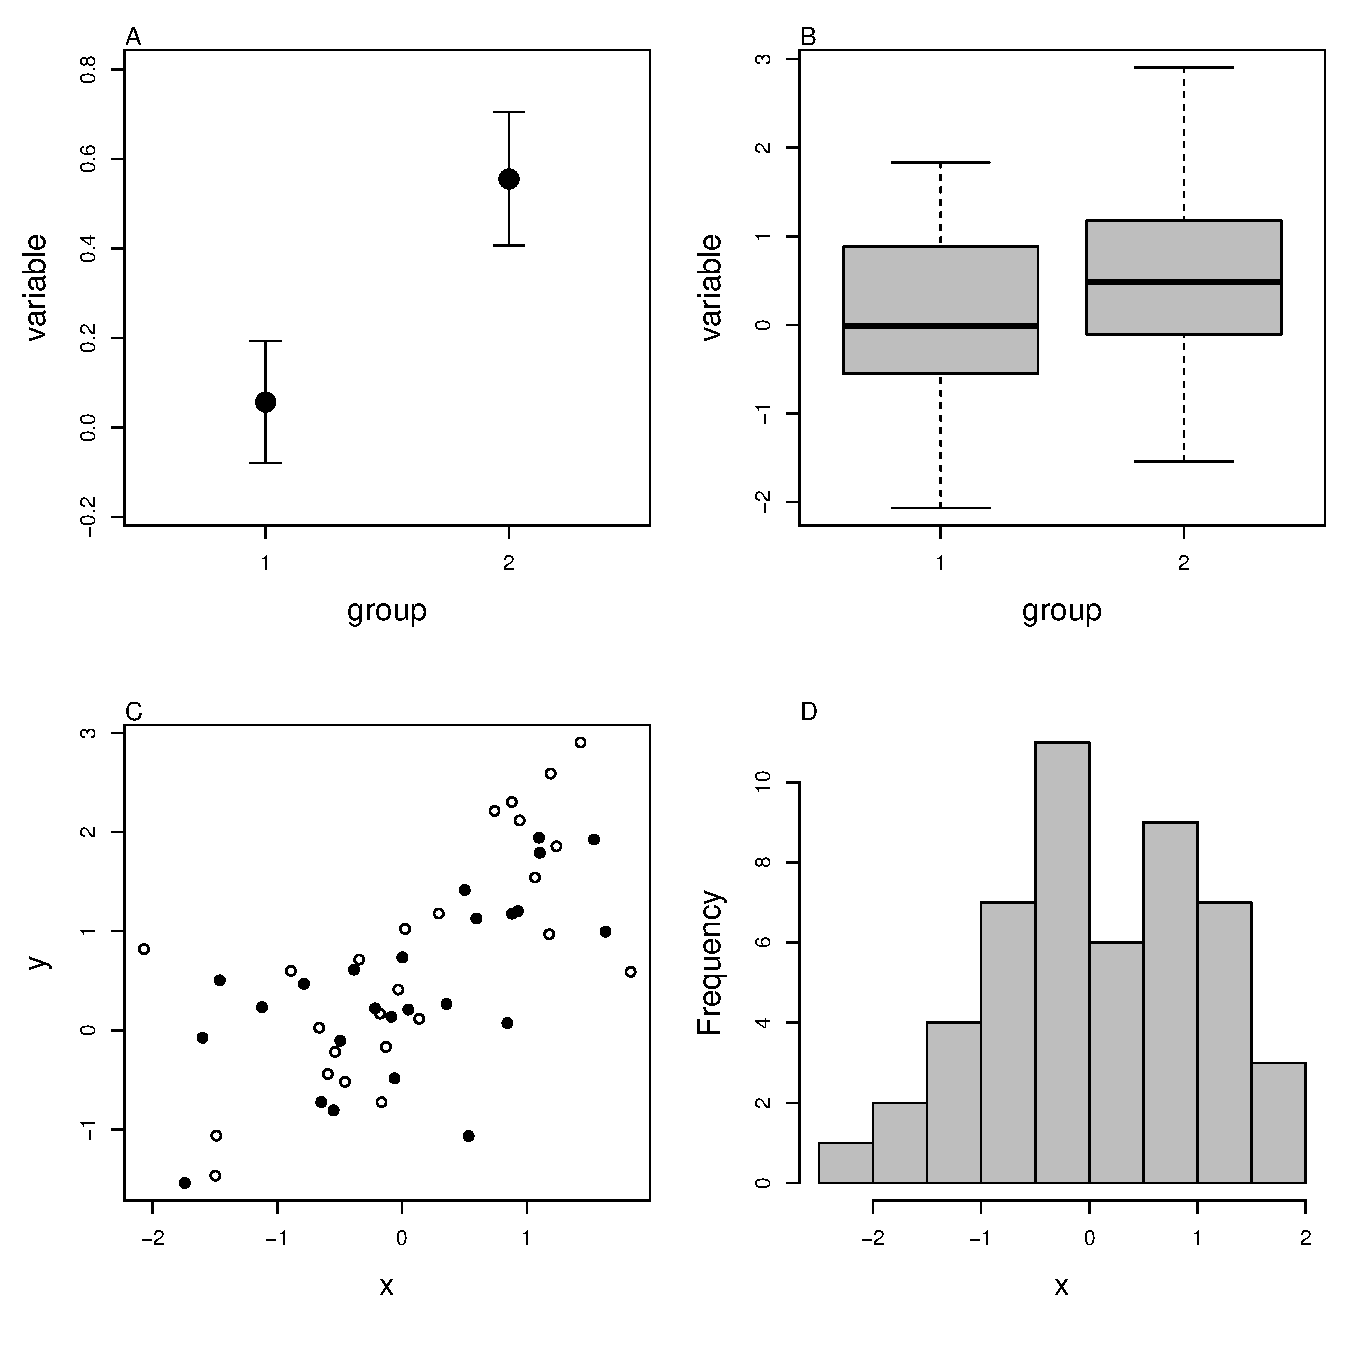
\includegraphics[width=0.9\textwidth]{fig_plot_type.pdf} 
 \caption{Four plot types that metaDigitise is designed to extract data from: A) mean and error plot, B) box plot, C) scatter plot and D) histogram. Data is taken from the iris dataset in R. A and B are plotted with the whole dataset, C and D are just the data for the species setosa.}
\label{fig:plot_type}
\end{figure}

\section{Functionality}
There is one main function in the package metaDigitise, which interactively takes the user through the process of extracting figures from graphs.

\subsection{Bulk Digitisation}
metaDigitise was created with the idea that the user would have multiple images to extract from. It therefore operates in the same way whether the user has one or multiple images. It assumes that the user has put all the figures needed for extraction in one parent directory. It first creates a new directory `caldat' inside this parent directory, in which calibration files are saved (see below). 

It then prompts the user to select whether they want to extract from new images, import previously extracted data or edit previously extracted data. Extracting from new images takes the user through the steps outlined below, figure by figure, giving the user the option to quit the process after each figure. If this process has already been started when the user starts metaDigitise, then it starts where the user left off. Similarly if the user adds new images to the parent directory after all other images are extracted (or part way through), the new images will be integrated into the extraction procedure. After extraction (or upon quitting the function), the extracted data will be returned. %% explain summary etc


If the process of data extraction has been finished, or the user wants to reimport summary or processed data ...






\subsection{Figure Rotation}
Figure may have been extracted from old publications, for example from scanned images, and so are not perfectly orientated on the image. This will make the calibration of the points in the figure from the image problematic. metaDigitise allows users to rotate the image. By clicking two points on the x-axis, metaDigitse calculates the angle needed to rotate the image so the x-axis is horizontal, and rotates it. (Figure \ref{fig:rotate}A,B)

\begin{figure}[!h] 
%\onehalfspacing
 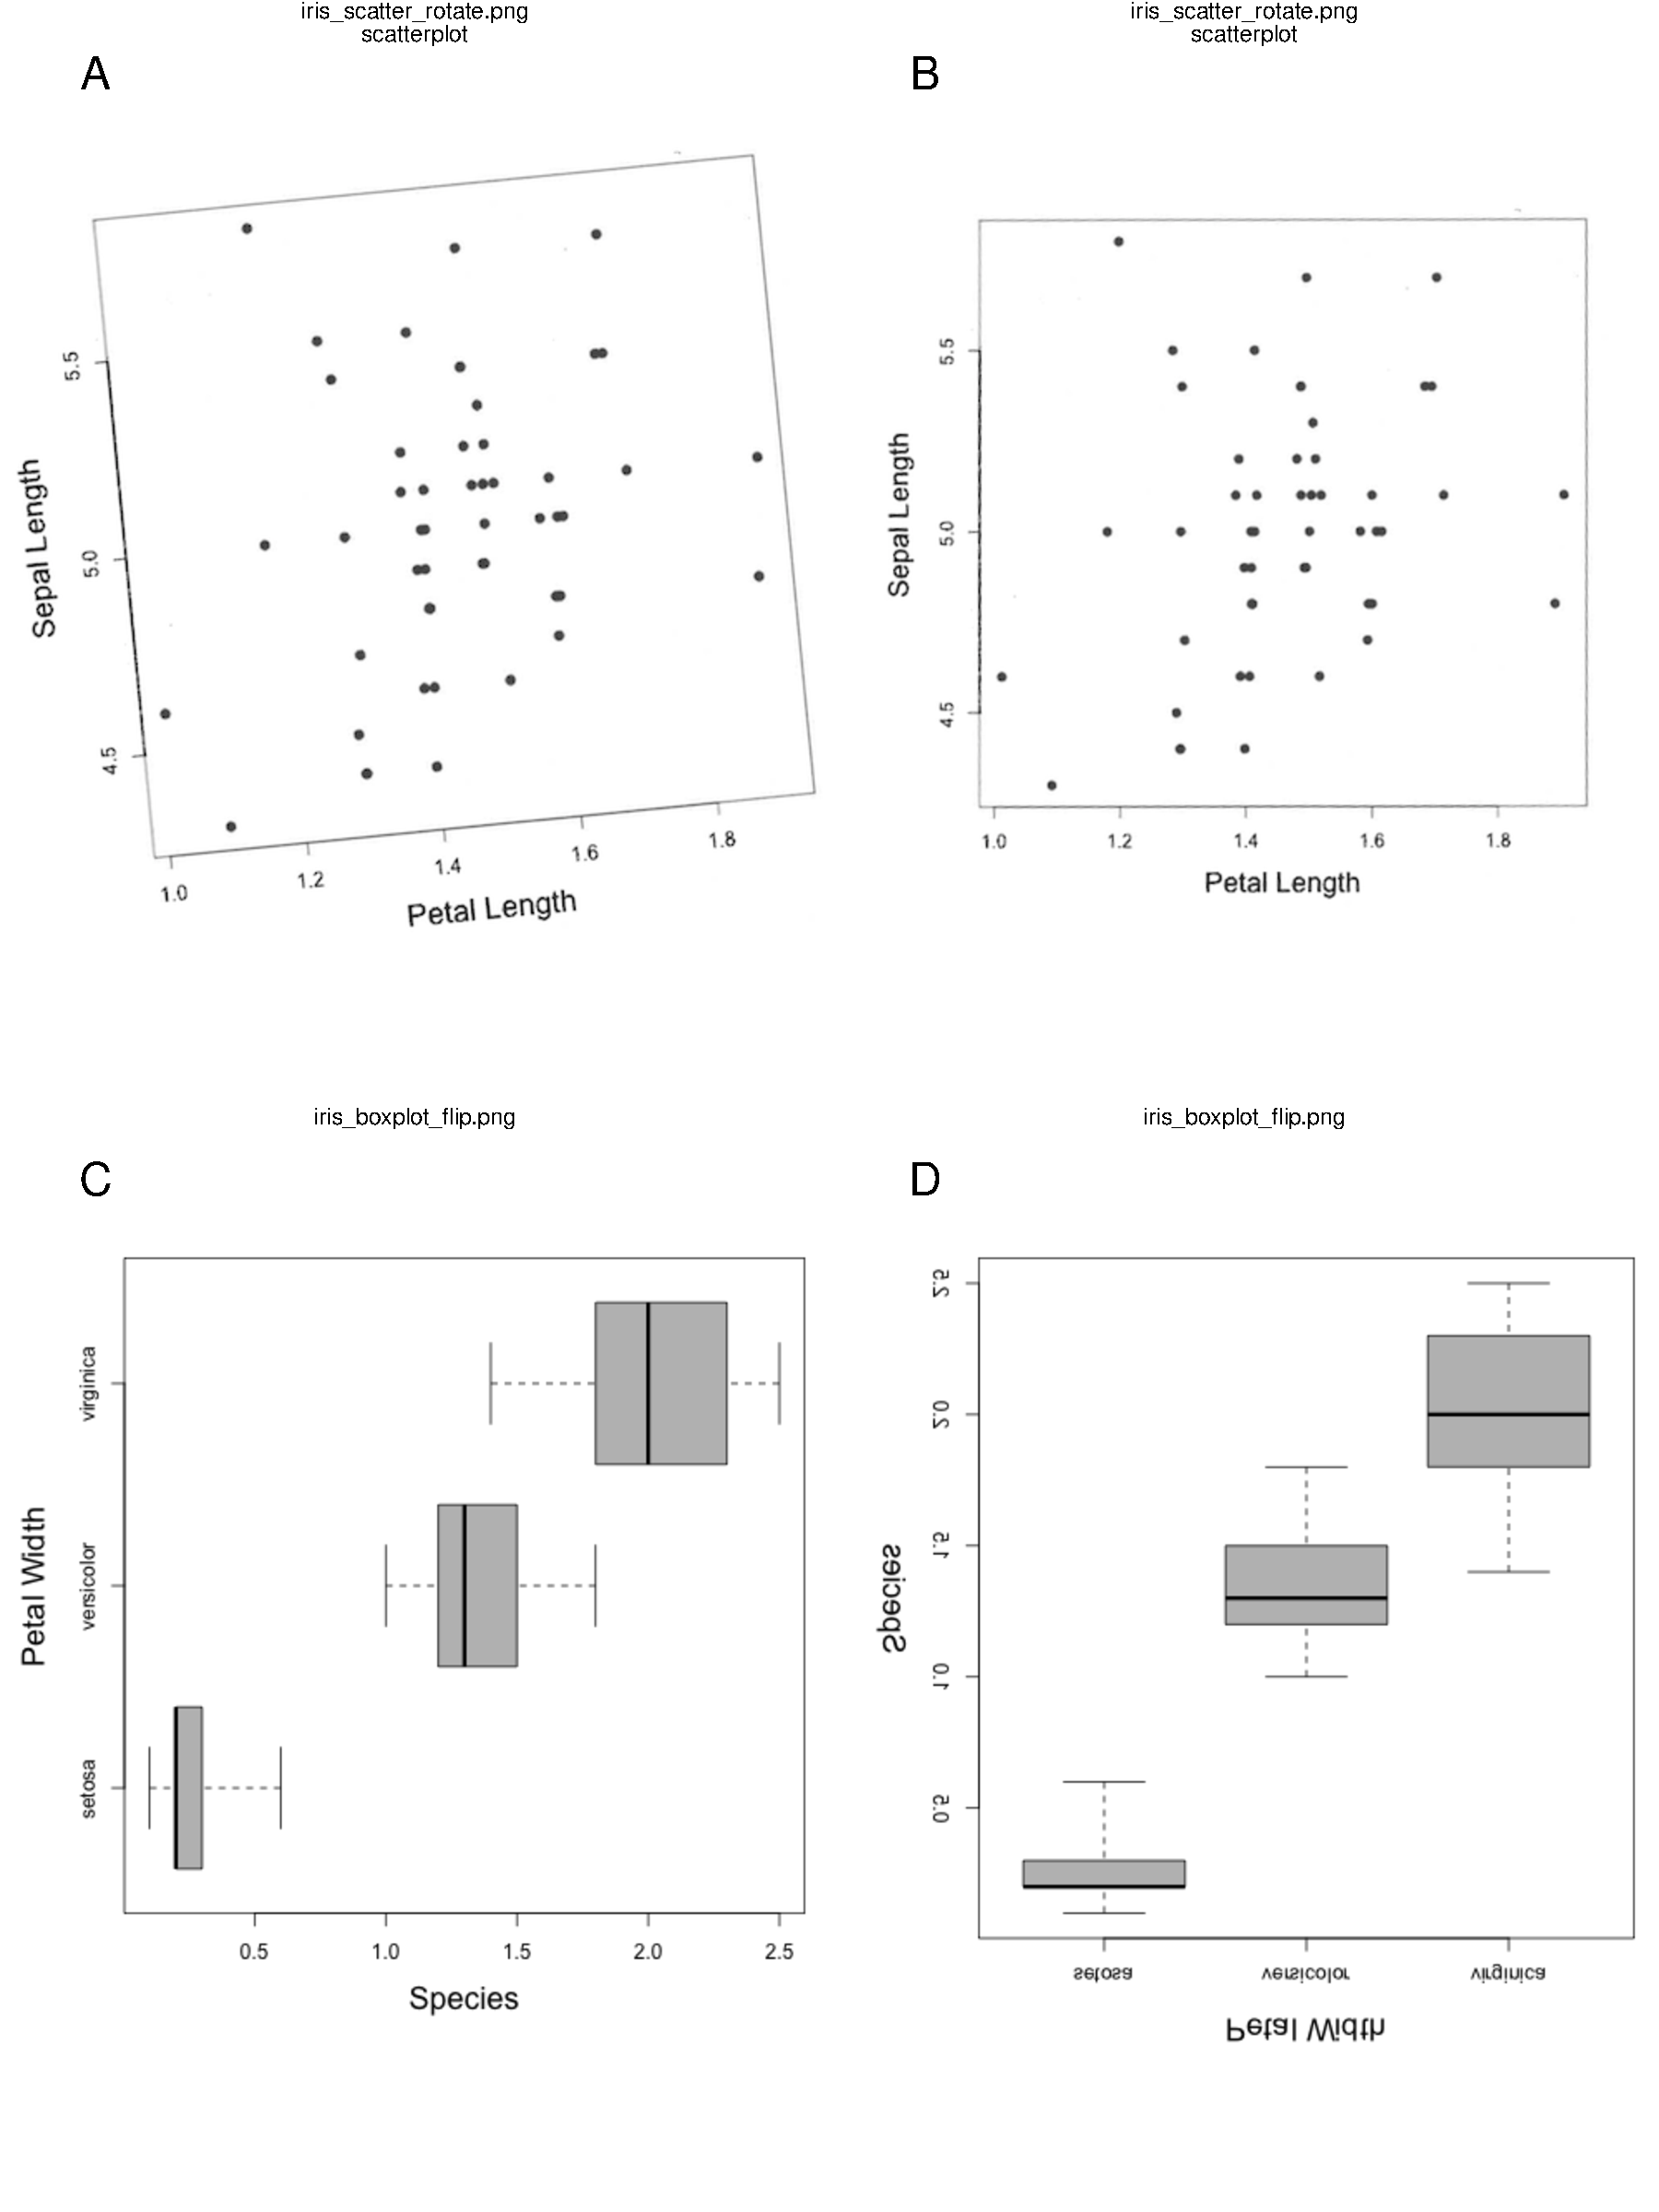
\includegraphics[width=0.9\textwidth]{fig_rotate.pdf} 
 \caption{Figure rotation. A) and B) show how non-aligned imaged can be realigned through user defined rotation. C) and D) show show figures can be re-orientated so as to aid data input.}
\label{fig:rotate}
\end{figure}

Furthermore, in some figures mean and error, boxplots or histograms may be presented with horizontal bars. metaDigitise assumes that the bars are vertical, but allows the user to flip the image so that the bars are vertical (Figure \ref{fig:rotate}C,D).


\subsection{Calibration}
metaDigitise requires the user to calibrate the axes in the figure. To do this the user is required to click on two known points on the axis in question, and then enter the value of those points in the figure (Figure \ref{fig:calibrate}). Using this information, metaDigitise then calculates the value of any clicked points in terms of the figure axes. In the case of mean and error plots and box plots, it calibrates only the y axis (assuming the x axis is redundant). For scatter plots and histograms both axes are calibrated.


\begin{figure}[!h] 
%\onehalfspacing
 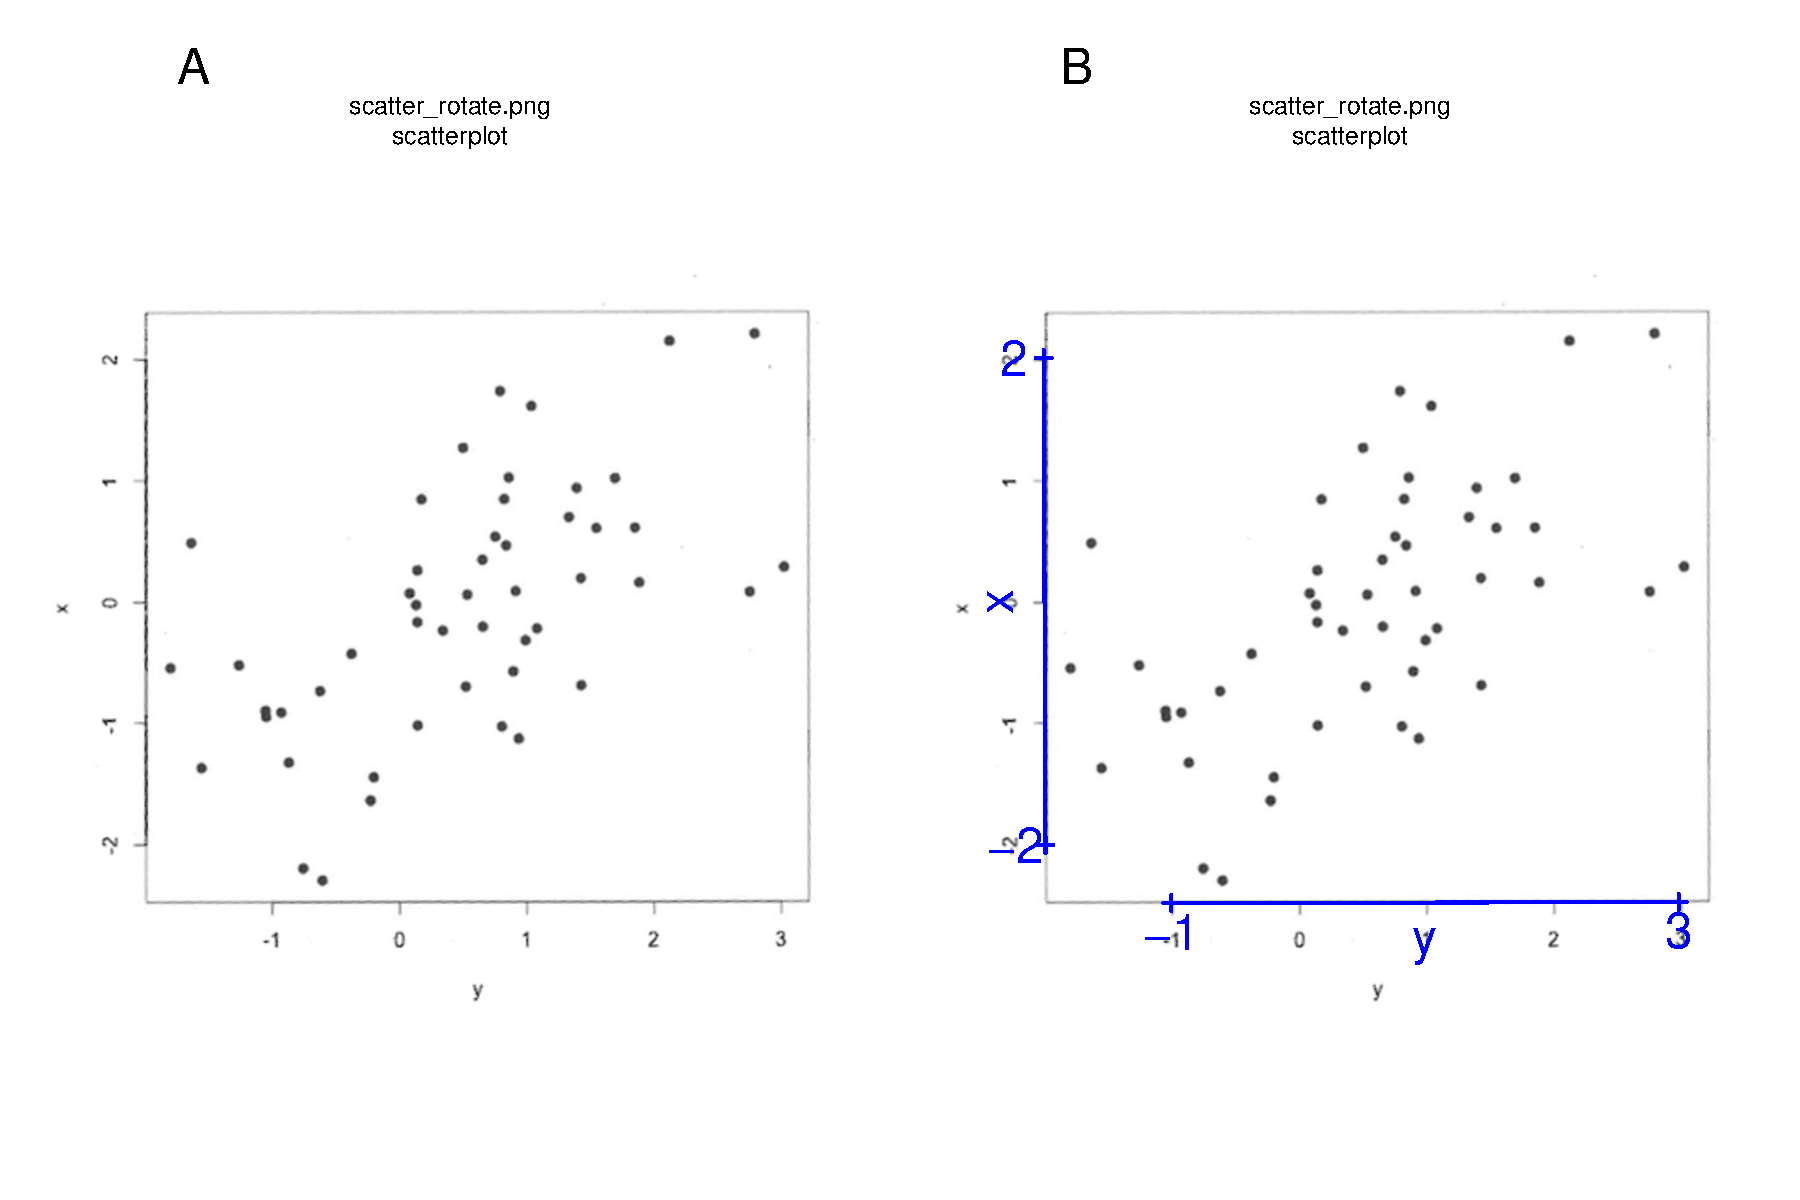
\includegraphics[width=0.9\textwidth]{fig_calibrate.pdf} 
 \caption{Axis calibration. The user defines two points on each axis and labels them according to the values shown in the figure.}
\label{fig:calibrate}
\end{figure}

\subsection{Plot Types}
metaDigitise recognises 4 main types of plot; Mean and error plots, box plots, scatter plots and histograms, shown in Figure \ref{fig:plot_type}. 

\begin{figure}[!h] 
%\onehalfspacing
 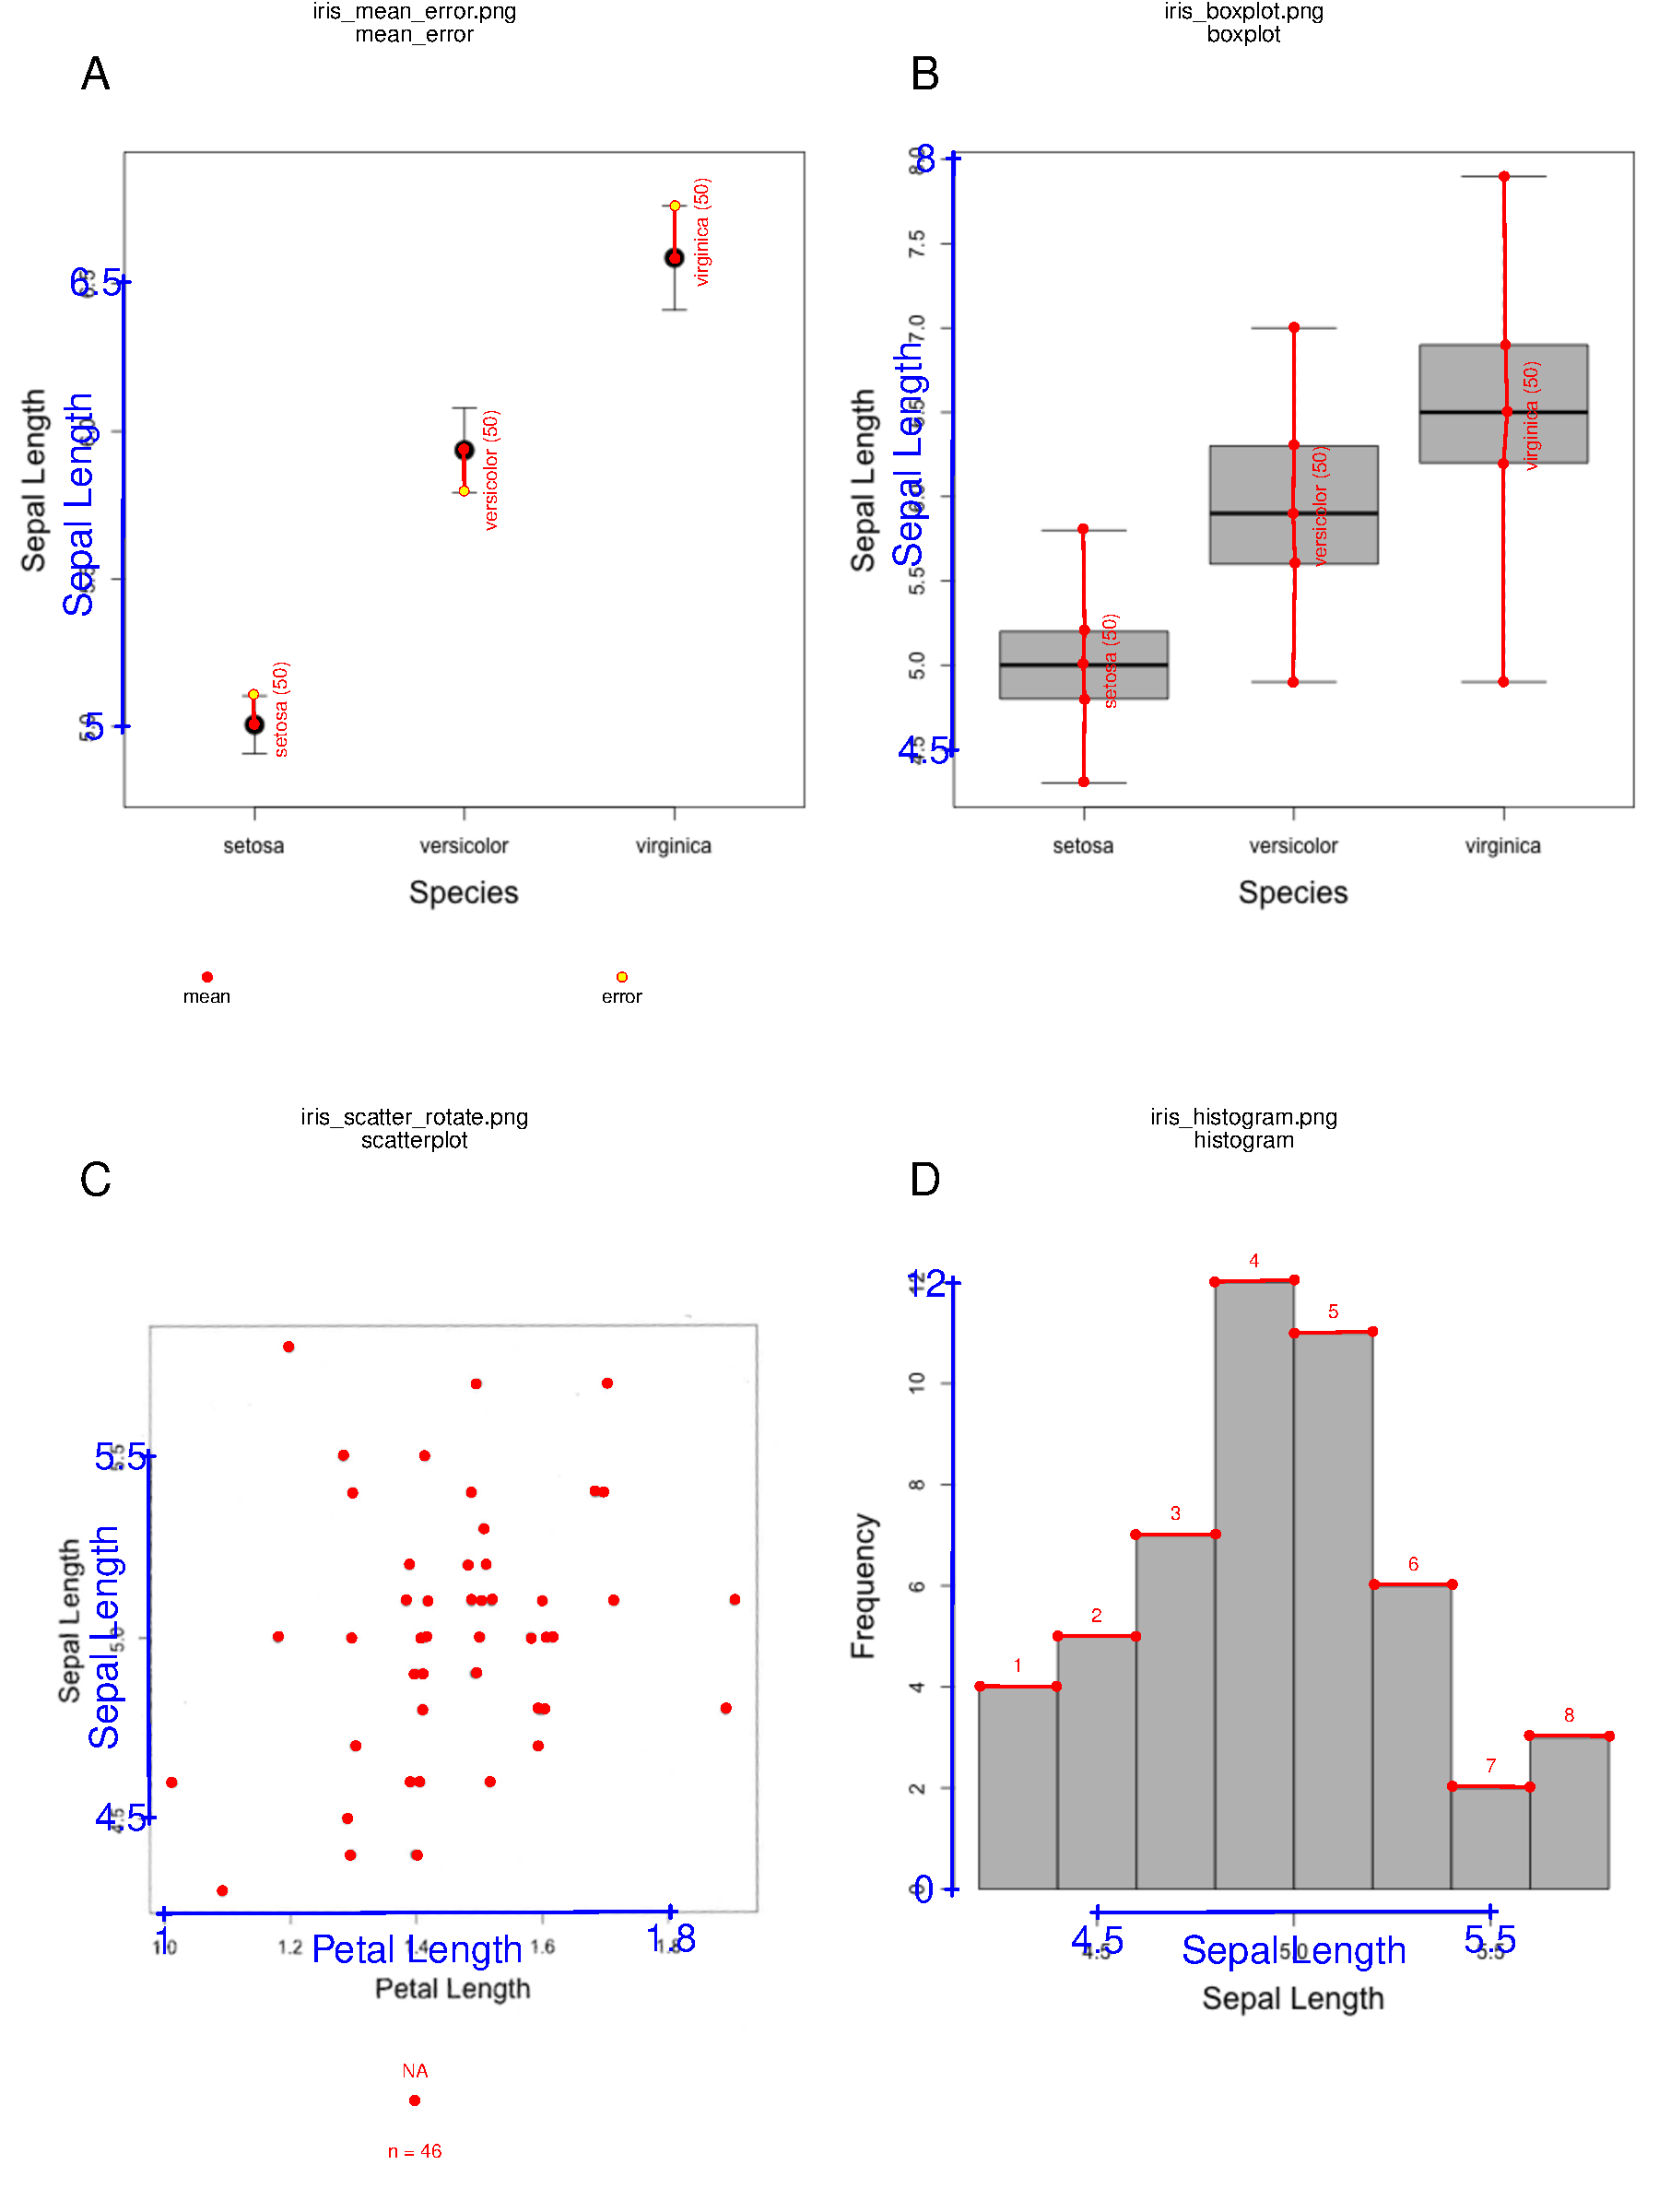
\includegraphics[width=0.9\textwidth]{fig_all_extract.pdf} 
 \caption{Demonstration of data extraction from different plot types}
\label{fig:all_extract}
\end{figure}

\subsubsection{Mean and error plots} 
metaDigitise prompts the user to enter groups names and allows the user to enter sample sizes, which are used in downstream processing. The user is then prompted to click on an error bar followed by the mean. Error bars above or below the mean can be clicked - sometimes one is clearer than the other. metaDigitise assumes that the error bars are symmetrical. Where the user has clicked the error is displayed in a different colour to the mean (Figure \ref{fig:all_extract}A). The user can subsequently add more groups or remove groups.


\subsubsection{Box plots}
 metaDigitise prompts the user to enter groups names and allows the user to enter sample sizes, which are used in downstream processing. The user is then prompted to click on the maximum, upper quartile, median, lower quartile and minimum. metaDigitise will check that the maximum is greater than the minimum, and return an warning if that is not the case. The user can subsequently add more groups or remove groups.

\subsubsection{Scatter plots}
 metaDigitise prompts the user to enter groups names and then to click on points. Points added by mistake can be deleted. The user can subsequently add groups, edit groups (add or remove points) or delete groups. Different groups are plotted in different colours and shapes, with a legend at the bottom of the figure (Figure \ref{fig:all_extract}C). The x and y coordinates are returned.


\subsubsection{Histograms}
metaDigitise prompts the user to enter groups names and then to click on the top corners of each bar. bars can subsequently be deleted. MetaDigitise then calculates the midpoint and the frequency for each bar. 


\subsection{Summary Data}
From all plot types, metaDigitise summarises the data form the figure to a mean, standard deviation and sample size, for each identified group. These are the summary statistical needed to create all relevant statistics for a meta-analysis. In the case of scatter plots, metaDigitise also returns the correlation coefficient between the points within each identified group. 

%%% Equations for mean and sd



%% pooled stats: 
% \begin{align}
% \mu _{X}&={\frac {\sum _{i}{N_{X_{i}}\mu _{X_{i}}}}{\sum _{i}{N_{X_{i}}}}}
% \\
% \sigma _{X}&={\sqrt {{\frac {1}{\sum _{i}{N_{X_{i}}-1}}}\left(\sum _{i}{\left[(N_{X_{i}}-1)\sigma _{X_{i}}^{2}+N_{X_{i}}\mu _{X_{i}}^{2}\right]}-\left[\sum _{i}{N_{X_{i}}}\right]\mu _{X}^{2}\right)}}
% \end{align}

\section{Reproducibility}

\subsection{Plotting data extraction}
check extraction

\subsection{Editing data extraction}
Including addition of N later


\section{Example}
%% scatterplot from airquality data


\section{Testing}
%% simulated data
%% x people doing y plots



\end{document}

